\documentclass[12pt]{article}

% Layout.
\usepackage[top=1in, bottom=0.75in, left=1in, right=1in, headheight=1in, headsep=6pt]{geometry}

% Fonts.
\usepackage{mathptmx}
\usepackage[scaled=0.86]{helvet}
\renewcommand{\emph}[1]{\textsf{\textbf{#1}}}

% TiKZ.
\usepackage{tikz, pgfplots}
\usetikzlibrary{calc}
\pgfplotsset{my style/.append style={axis x line=middle, axis y line=
middle, xlabel={$x$}, ylabel={$y$}, axis equal }}

% Misc packages.
\usepackage{amsmath,amssymb,latexsym}
\usepackage{graphicx}
\usepackage{array}
\usepackage{xcolor}
\usepackage{multicol}

% Commands to set various header/footer components.
\makeatletter
\def\doctitle#1{\gdef\@doctitle{#1}}
\doctitle{Use {\tt\textbackslash doctitle\{MY LABEL\}}.}
\def\docdate#1{\gdef\@docdate{#1}}
\docdate{Use {\tt\textbackslash docdate\{MY DATE\}}.}
\def\doccourse#1{\gdef\@doccourse{#1}}
\let\@doccourse\@empty
\def\docscoring#1{\gdef\@docscoring{#1}}
\let\@docscoring\@empty
\def\docversion#1{\gdef\@docversion{#1}}
\let\@docversion\@empty
\makeatother

% Headers and footers layout.
\makeatletter
\usepackage{fancyhdr}
\pagestyle{fancy}
\fancyhf{} % Clears all headers/footers.
\lhead{\baselineskip 30pt
\emph{\@doctitle\hfill\@docdate}
\ifnum \value{page} > 1\relax\else\\
\emph{Name: \rule{3.5in}{1pt}\ \hfill
%Class (circle): \ \  Sync. \hfill Online%\@docscoring
}
\fi}
\rfoot{\emph{\@docversion}}
\lfoot{\emph{\@doccourse}}
\cfoot{\emph{\thepage}}
\renewcommand{\headrulewidth}{0pt}%
\makeatother

% Paragraph spacing
\parindent 0pt
\parskip 6pt plus 1pt

% A problem is a section-like command. Use \problem{5} to
% start a problem worth 5 points.
\newcounter{probcount}
\newcounter{subprobcount}
\setcounter{probcount}{0}
\newcommand{\problem}[1]{%
\par
\addvspace{4pt}%
\setcounter{subprobcount}{0}%
\stepcounter{probcount}%
\makebox[0pt][r]{\emph{\arabic{probcount}.}\hskip1ex}\emph{[#1 points]}\hskip1ex}
\newcommand{\thesubproblem}{\emph{\alph{subprobcount}.}}

% Subproblems are an enumerate-like environment with a consistent
% numbering scheme. 
% Use \begin{subproblems}\item...\item...\end{subproblems}
\newenvironment{subproblems}{%
\begin{enumerate}%
\setcounter{enumi}{\value{subprobcount}}%
\renewcommand{\theenumi}{\emph{\alph{enumi}}}}%
{\setcounter{subprobcount}{\value{enumi}}\end{enumerate}}

% Blanks for answers in normal and math mode.
\newcommand{\blank}[1]{\rule{#1}{0.75pt}}
\newcommand{\mblank}[1]{\underline{\hspace{#1}}}
\def\emptybox(#1,#2){\framebox{\parbox[c][#2]{#1}{\rule{0pt}{0pt}}}}

% Misc.
\renewcommand{\d}{\displaystyle}
\newcommand{\ds}{\displaystyle}
\def\bc{\begin{center}}
\def\ec{\end{center}}


\doctitle{Math 251: Section 4.7 Set up + More Trig}
\docdate{Recitation Week 10}
\doccourse{UAF Calculus I}
%\docversion{v-practice}
%\docscoring{\blank{0.8in} / 12}

\begin{document}
\addtolength\itemsep{-1mm}

This page helps you set up some of the more challenging problems from Section 4.7. Note that the point is not to work the problems but to get them set up.
\begin{enumerate}
\item Technique: Use units to help you. 
\begin{enumerate}
	\item If $a=20$ mph and $b=15$ miles, what are the units of $ab$, $a/b$, $b/a$?\\
	\item If $a=20$ mph and $c=10$ dollars per hour, what are the units of $ab$, $a/b$, $b/a$?\\
\end{enumerate}

\item (4.7.326) You can run at a speed of 6 mph and swim at a speed of 3 mph and are located on the shore 4 miles east of an island that is 1 mile north of the shoreline How far should you run west to minimize the time needed to reach the island?

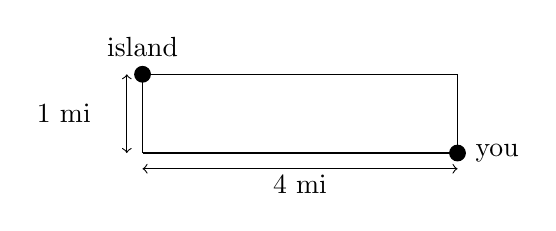
\begin{tikzpicture}
\draw (0,0) -- (0,1) -- (4,1) -- (4,0) -- (0,0);
\draw [<->] (0,-.2) -- (4,-0.2);
\node at (2,-.4){$4$ mi};
\draw [<->] (-.2,0) -- (-0.2,1);
\node at (-1,0.5){$1$ mi};
\node[circle, draw,fill=black, inner sep=2pt, minimum size=2pt] at (4,0)[label=right: you]{};
\node[circle, draw,fill=black, inner sep=2pt, minimum size=2pt] at (0,1)[label=above: island]{};
%\node[circle, draw, inner sep=2pt, minimum size=2pt] at (0,0)[label=left: A ]{};
%\node[circle, draw, inner sep=2pt, minimum size=2pt] at (1.5,0)[label=above: B]{};
\end{tikzpicture}


\begin{enumerate}
	\item What quantity are you minimizing or maximizing and what units does it have? Give this quantity a variable.
	\item Draw a sample run-to-swim path in the picture and pick a variable(s). (Hint: Be thoughtful about your choice.)
	\item	Write you quantity in part (a) as a function on one variable.
\end{enumerate}
\vfill
\item (4.7.330 \& 331) A limousine gets $m(v)=\frac{120-2v}{5}$ mi/gal at speed $v$, the chauffeur costs \$15 per hour, and gasoline is \$3.50 per gallon. Find the cost per mile at speed $v.$
\begin{enumerate}
	\item You are supposed to write \emph{something} as a function of speed $v.$ What is that \emph{something}? What units does it have? Pick a letter to represent this something.
	\item Assuming you must consider both fuel costs (gasoline) and personnel costs (chauffeur), answer the question.
\end{enumerate}
\vfill
\newpage
\item You are a manager of an apartment complex with 50 units. When you set rent at \$800/month, all the apartments are rented. As you increase rent by \$25/month, one fewer apartment is rented. Maintenance costs run \$50/month for each occupied unit. What is the rent that maximizes the total amount of profit?
\begin{enumerate}
	\item What are you trying to maximize or minimize? What units does it have? Pick a variable to represent it.
	\item What is the independent variable? Pick a variable to represent this, too.
	\item Now write the variable in (a) as a function of the variable in $b$.
	\end{enumerate}
\vfill
\item Go back to problems 1-3 and determine a domain for each problem.
\item Fill out the unit circle. Note the $30^o$ has been done for you. Use it to solve $\tan \theta =-1.$\\
\includegraphics[scale=0.5]{blank-unit-circle.pdf}
\end{enumerate}

\end{document}